\section{First Models}
\label{sec:first_models}

\subsection{Bag of Words}
\label{sec:bag_of_words}
From the examination of the data in Section \ref{sec:word_frequency}, a bag-of-words classifier seems plausible. Through a direct comparison of the frequencies with which each author uses the words in a given sentence, a prediction may be formed.

Let $\phi_w^a$ be the number of occurrences of some word $w$ in the corpus of sentences attributed to author $a$. The estimated probability of an author's usage of a word, $w^*$, is given by:

\begin{equation*}
p_{w*}^a = \frac{\phi_w^a}{\sum\limits_{w} \phi_w^a}
\end{equation*}

The estimated probability of a sentence, $s$, is given by:

\begin{align*}
p_{s}^a &= \prod\limits_{w\in s} p_{w}^a \\
log(p_{s}^a &)= \sum\limits_{w\in s} log(p_{w}^a)
\end{align*}

During prediction, however, it is likely that certain words will not have occurred in the training data: a "miss". An intuitive way to handle this is to score authors first on the number of words they "hit", and then by the probability of those words. Denoting the words used by each author in the training set as $W_a$ and the set of authors $A$, the following scoring mechanism is introduced:

\begin{align*}
score(s,a) &= \sum\limits_{w\in s}
\begin{cases}
log(p_{w}^a) & w\in W_a \\
0 & w \not\in W_a
\end{cases}\\
hits(s,a) &= \sum\limits_{w\in s}
\begin{cases}
1 & w\in W_a \\
0 & w \not\in W_a
\end{cases}\\
cands(s) &= a^* \in A : hits(s,a^*) = \max_a(hits(s,a))\\
winner(s) &= \underset{a}{\arg\max}(score(s,a))\quad \forall a \in cands(s)
\end{align*}

Running this model on the training set with 3 cross-validation passes (such that each third of the training data is predicted based on a model trained on the remaining two-thirds) yields the confusion matrix and accuracy in Table \ref{tab:bow_cw}. Log-loss metrics are not available for this model as it doesn't produce output probabilities, only binary classifications.

\begin{table}[h]
\centering
\begin{tabular}{m{1cm}|m{1cm}|m{1cm}|m{1cm}|m{0cm}}
\multicolumn{1}{m{1cm}}{} & \multicolumn{1}{m{1cm}}{EAP} & \multicolumn{1}{m{1cm}}{HPL} & \multicolumn{1}{m{1cm}}{MWS} &\\[5pt]
\cline{2-4}
EAP & 4910 & 630 & 760 & \\[5pt]
\cline{2-4}
HPL & 476 & 3774 & 283 & \\[5pt]
\cline{2-4}
MWS & 615 & 381 & 3834 & \\[5pt]
\cline{2-4}
\end{tabular}
\caption{Results for bag-of-words classifier, stemming and lemmatisation enabled.\\Accuracy: 80\%}
\label{tab:bow_cw}
\end{table}

\subsection{Forest}
\label{sec:forest}

\subsection{Windowed Neural Network}
In order to recognise tell-tale structures in the way sentences are composed, a classifier must be able to examine words in context. By running a window over the sentence tokens, this can be achieved.

Using a word embedding of $d$ dimensions, a window of $n$ words is provided as the input to a neural network. These words are flattened into a $d \times n$ wide layer, and fed through some number of hidden Relu units before being fed to a classifying output layer. This overall structure is described in Figure \ref{fig:win_nn_structure}.

\begin{figure}[h]
\def\layersep{2cm}
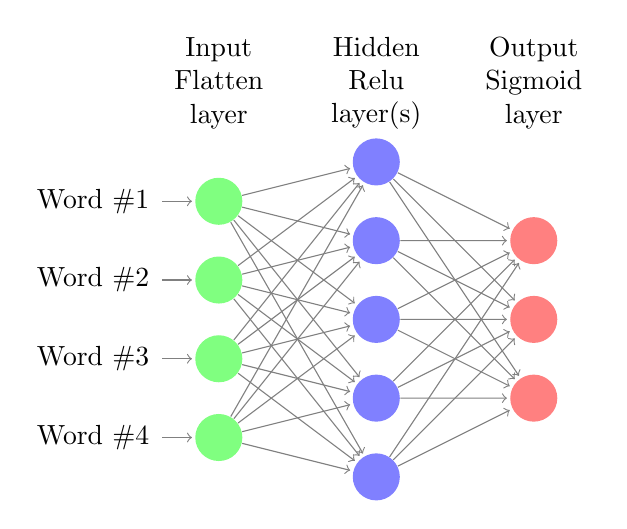
\begin{tikzpicture}[shorten >=1pt,->,draw=black!50, node distance=\layersep]
    \tikzstyle{every pin edge}=[<-,shorten <=1pt]
    \tikzstyle{neuron}=[circle,fill=black!25,minimum size=17pt,inner sep=0pt]
    \tikzstyle{input neuron}=[neuron, fill=green!50];
    \tikzstyle{output neuron}=[neuron, fill=red!50];
    \tikzstyle{hidden neuron}=[neuron, fill=blue!50];
    \tikzstyle{annot} = [text width=4em, text centered]

    % Draw the input layer nodes
    \foreach \name / \y in {1,...,4}
    % This is the same as writing \foreach \name / \y in {1/1,2/2,3/3,4/4}
        \node[input neuron, pin=left:Word \#\y] (I-\name) at (0,-\y) {};
        
    % Draw the hidden layer nodes
    \foreach \name / \y in {1,...,5}
        \path[yshift=0.5cm]
            node[hidden neuron] (H-\name) at (\layersep,-\y cm) {};

    % Draw the output layer node
    \foreach \name / \y in {1,...,3}
    	\path[yshift=-0.5cm]
            node[output neuron] (G-\name) at (2*\layersep,-\y cm) {};

    % Connect every node in the input layer with every node in the
    % hidden layer.
    \foreach \source in {1,...,4}
        \foreach \dest in {1,...,5}
            \path (I-\source) edge (H-\dest);

    % Connect every node in the hidden layer with the output layer
    \foreach \source in {1,...,5}
        \foreach \dest in {1,...,3}
            \path (H-\source) edge (G-\dest);

    % Annotate the layers
    \node[annot,above of=H-1, node distance=1cm] (hl) {Hidden Relu layer(s)};
    \node[annot,left of=hl] {Input Flatten layer};
    \node[annot,right of=hl] {Output Sigmoid layer};
\end{tikzpicture}
\caption{Windowed neural network structure}
\label{fig:win_nn_structure}
\end{figure}

The word embedding for this network may either be built on the training set itself or imported from a pre-trained model. The former may create a more subject-specific embedding since it is trained on relevant data; however the relatively small corpus size means that the spacial relationship between words may be weaker and the likelihood of missing words in the test data may be higher.

For this classifier, these embeddings are as described in Section \ref{sec:word2vec}.

In either case, it must be decided how to deal with words in the test data that do not exist in the word embedding. For the embedding built from the training set, unique words (that is, words that appear only once across all sentences) are replaced with a \textit{RARE} token. This creates an embedding for unique words, and when the model is run any words which do not exist in the embedding may be replaced with this token.

For the pre-trained model, inserting tokens is not possible. Instead words that do not exist within the embedding are replaced with a mean vector, $\vec{e}_{rare}$, derived from the embedding $E$, such that:

\begin{equation*}
\vec{e}_{rare} = \frac{1}{\lVert E \rVert} \sum\limits_{\vec{w} \in E}^{\lVert E \rVert} \vec{w}
\end{equation*}


Additionally test sentences with length less than the window size must be padded to at least that length; In this model, such sentences are being appended with the last word in the sentence until long enough.

The confusion matrices, log-losses and accuracies for this model under both encoder methods are shown in Table \ref{tab:window_res}.

\begin{table}[h]
\centering
\begin{subtable}{\columnwidth}
\centering
\begin{tabular}{m{1cm}|m{1cm}|m{1cm}|m{1cm}|m{0cm}}
\multicolumn{1}{m{1cm}}{} & \multicolumn{1}{m{1cm}}{EAP} & \multicolumn{1}{m{1cm}}{HPL} & \multicolumn{1}{m{1cm}}{MWS} &\\[5pt]
\cline{2-4}
EAP & 4504 & 773 & 1023 & \\[5pt]
\cline{2-4}
HPL & 1201 & 2632 & 700 & \\[5pt]
\cline{2-4}
MWS & 1206 & 543 & 3081 & \\[5pt]
\cline{2-4}
\end{tabular}
\caption{Encoding built from training data, stemming and lemmatisation enabled.\\Loss: 1.83 Accuracy: 65\%}
\end{subtable}\\
\vspace{1cm}
\begin{subtable}{\columnwidth}
\centering
\begin{tabular}{m{1cm}|m{1cm}|m{1cm}|m{1cm}|m{0cm}}
\multicolumn{1}{m{1cm}}{} & \multicolumn{1}{m{1cm}}{EAP} & \multicolumn{1}{m{1cm}}{HPL} & \multicolumn{1}{m{1cm}}{MWS} &\\[5pt]
\cline{2-4}
EAP & 4587 & 757 & 956 & \\[5pt]
\cline{2-4}
HPL & 1084 & 2885 & 564 & \\[5pt]
\cline{2-4}
MWS & 1019 & 525 & 3286 & \\[5pt]
\cline{2-4}
\end{tabular}
\caption{Pre-trained GloVe encoder, stemming and lemmatisation enabled.\\Loss: 1.90 Accuracy: 69\%}
\end{subtable}
\caption{Results for windowed neural net classifier.}
\label{tab:window_res}
\end{table}

\label{sec:dnn}

\subsection{RNN}
\label{sec:rnn}
  An obvious choice for textual input data was a recursive neural network.
  Tensorflow made it simple to write a model which allowed a choice of recursive
  cell (basic, LSTM or GRU) and so all three were investigated.  
  
  Figure \ref{fig:rnn-structure} shows the structure of the RNN. As recommended
  by one of the PhD student project advisors, outputs were generated from a
  dense network fed by the internal state of the recursive cell. This dense
  network used a sigmoid activation function so that its outputs ranged between
  0 and 1 and so could learn confidences for each author. 
  
  \begin{figure}[ht]
    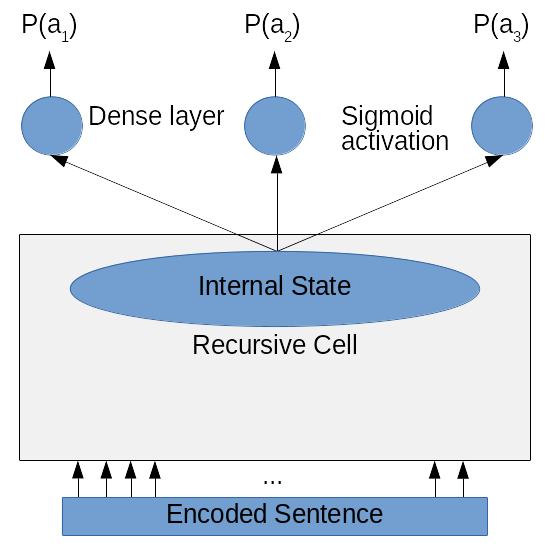
\includegraphics[width=0.45\textwidth]{Figures/rnn.png}
    \caption{Recursive neural network structure}
    \label{fig:rnn-structure}
  \end{figure}
  
    The RNN was trained using cross-entropy loss and an Adam optimizer. Data
    were fed in using randomized batches so that the data could all fit into GPU
    memory and to improve generalisation performance. Initially a batch size of
    100 sentences was used but this led to over fitting of each batch even for
    relatively small networks. When the batch size was increased to 200 this
    problem lessened significantly because this larger batch provided a much
    more representative sample of the dataset. 
    
    In early testing it was predictably found that the basic RNN cell was out
    performed by LSTM and GRU cells. Less obviously, changing the weights
    initialiser from Xavier (Tensorflow default) to He initialisation harmed
    performance. 
    
    The prediction accuracy on the training dataset was observed to be slightly
    higher than on the test dataset, particularly as the number of neurons used
    in the recursive cell was increased. However, this difference remained
    constant as networks were made larger and trained for longer - not showing
    the characteristic increase in testing error as models overfit training
    data. As a result of this behaviour early stopping was not implemented.
    However the overfitting was combatted by imposing dropout during training.  
    
    Early experimentation also investigated the format of the encoded sentences.
    A very significant (almost 30\%) accuracy improvement was gained by using
    whole padded sentences instead of short windows into sentences. Presumably
    the recursive networks were remembering some features throughout the
    sentence. Stemming and stop word removal were also tested and found to have
    a small detrimental effect. 
    
    By the end of this early phase, the RNN achieved 68\% accuracy, with similar
    precision and recall scores: indicating no bias towards one class over
    another. 
    
   
